\documentclass{standalone}
\usepackage{tikz}
\usetikzlibrary{patterns, positioning}

\begin{document}
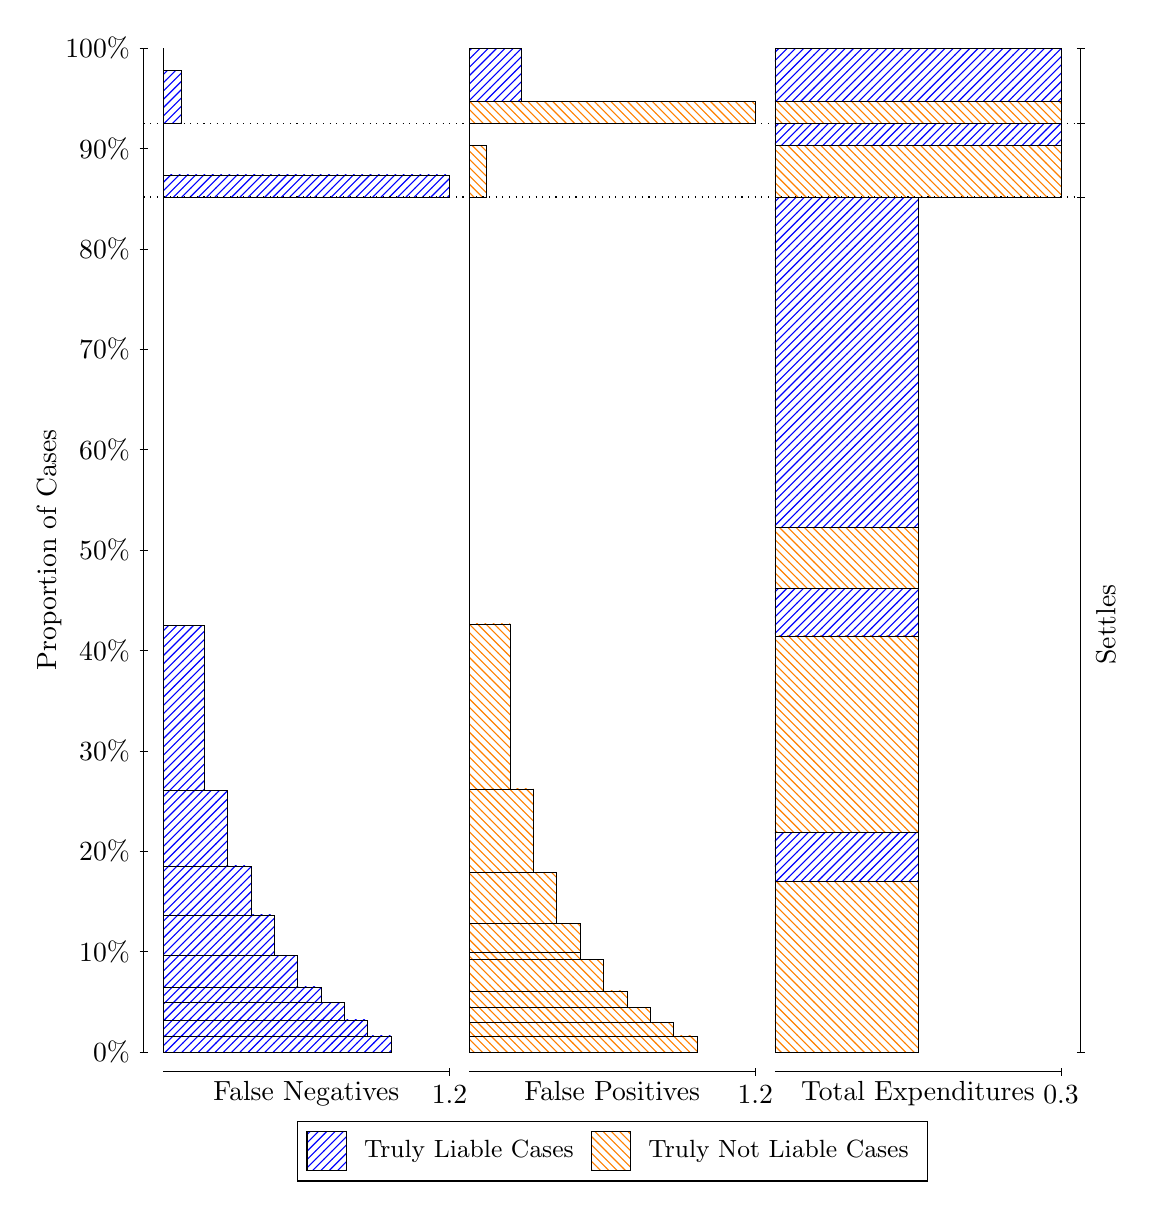
\begin{tikzpicture}
\draw[black, very thin] (1.5,1.75) -- (1.5,14.5);
\node[rotate=90, anchor=center] at (0.3, 8.125) {Proportion of Cases};
\draw[black, very thin] (1.45,1.75) -- (1.55,1.75);
\node[anchor=east] at (1.45, 1.75) {0\%};
\draw[black, very thin] (1.45,3.025) -- (1.55,3.025);
\node[anchor=east] at (1.45, 3.025) {10\%};
\draw[black, very thin] (1.45,4.3) -- (1.55,4.3);
\node[anchor=east] at (1.45, 4.3) {20\%};
\draw[black, very thin] (1.45,5.575) -- (1.55,5.575);
\node[anchor=east] at (1.45, 5.575) {30\%};
\draw[black, very thin] (1.45,6.85) -- (1.55,6.85);
\node[anchor=east] at (1.45, 6.85) {40\%};
\draw[black, very thin] (1.45,8.125) -- (1.55,8.125);
\node[anchor=east] at (1.45, 8.125) {50\%};
\draw[black, very thin] (1.45,9.4) -- (1.55,9.4);
\node[anchor=east] at (1.45, 9.4) {60\%};
\draw[black, very thin] (1.45,10.675) -- (1.55,10.675);
\node[anchor=east] at (1.45, 10.675) {70\%};
\draw[black, very thin] (1.45,11.95) -- (1.55,11.95);
\node[anchor=east] at (1.45, 11.95) {80\%};
\draw[black, very thin] (1.45,13.225) -- (1.55,13.225);
\node[anchor=east] at (1.45, 13.225) {90\%};
\draw[black, very thin] (1.45,14.5) -- (1.55,14.5);
\node[anchor=east] at (1.45, 14.5) {100\%};

\draw[black, very thin] (13.4,1.75) -- (13.4,14.5);
\draw[black, very thin] (13.35,1.75) -- (13.45,1.75);
\node[anchor=west] at (13.35, 1.75) {};
\draw[black, very thin] (13.35,12.608) -- (13.45,12.608);
\node[anchor=west] at (13.35, 12.608) {};
\draw[black, very thin] (13.35,13.546) -- (13.45,13.546);
\node[anchor=west] at (13.35, 13.546) {};
\draw[black, very thin] (13.35,14.5) -- (13.45,14.5);
\node[anchor=west] at (13.35, 14.5) {};

\draw[black, very thin, pattern color=blue, pattern=north east lines] (1.75,1.75) rectangle (4.6418,1.9541);
\draw[black, very thin, pattern color=blue, pattern=north east lines] (1.75,1.9541) rectangle (4.3452,2.1573);
\draw[black, very thin, pattern color=blue, pattern=north east lines] (1.75,2.1573) rectangle (4.0486,2.3803);
\draw[black, very thin, pattern color=blue, pattern=north east lines] (1.75,2.3803) rectangle (3.752,2.5769);
\draw[black, very thin, pattern color=blue, pattern=north east lines] (1.75,2.5769) rectangle (3.4554,2.9748);
\draw[black, very thin, pattern color=blue, pattern=north east lines] (1.75,2.9748) rectangle (3.1588,3.4918);
\draw[black, very thin, pattern color=blue, pattern=north east lines] (1.75,3.4918) rectangle (2.8622,4.1127);
\draw[black, very thin, pattern color=blue, pattern=north east lines] (1.75,4.1127) rectangle (2.5656,5.0675);
\draw[black, very thin, pattern color=blue, pattern=north east lines] (1.75,5.0675) rectangle (2.269,7.1707);
\draw[black, very thin, pattern color=orange, pattern=north west lines] (1.75,7.1707) rectangle (1.75,12.608);
\draw[black, very thin, pattern color=blue, pattern=north east lines] (1.75,12.608) rectangle (5.3833,12.889);
\draw[black, very thin, pattern color=orange, pattern=north west lines] (1.75,12.889) rectangle (1.75,13.546);
\draw[black, very thin, pattern color=blue, pattern=north east lines] (1.75,13.546) rectangle (1.9724,14.218);
\draw[black, very thin, pattern color=orange, pattern=north west lines] (1.75,14.218) rectangle (1.75,14.5);
\draw[black, very thin, pattern color=orange, pattern=north west lines] (5.6333,1.75) rectangle (8.5252,1.9551);
\draw[black, very thin, pattern color=orange, pattern=north west lines] (5.6333,1.9551) rectangle (8.2286,2.1304);
\draw[black, very thin, pattern color=orange, pattern=north west lines] (5.6333,2.1304) rectangle (7.932,2.3169);
\draw[black, very thin, pattern color=orange, pattern=north west lines] (5.6333,2.3169) rectangle (7.6354,2.5263);
\draw[black, very thin, pattern color=orange, pattern=north west lines] (5.6333,2.5263) rectangle (7.3388,2.922);
\draw[black, very thin, pattern color=orange, pattern=north west lines] (5.6333,2.922) rectangle (7.0422,3.018);
\draw[black, very thin, pattern color=orange, pattern=north west lines] (5.6333,3.018) rectangle (7.0422,3.3806);
\draw[black, very thin, pattern color=orange, pattern=north west lines] (5.6333,3.3806) rectangle (6.7456,4.0299);
\draw[black, very thin, pattern color=orange, pattern=north west lines] (5.6333,4.0299) rectangle (6.449,5.09);
\draw[black, very thin, pattern color=orange, pattern=north west lines] (5.6333,5.09) rectangle (6.1524,7.1869);
\draw[black, very thin, pattern color=blue, pattern=north east lines] (5.6333,7.1869) rectangle (5.6333,12.608);
\draw[black, very thin, pattern color=orange, pattern=north west lines] (5.6333,12.608) rectangle (5.8558,13.264);
\draw[black, very thin, pattern color=blue, pattern=north east lines] (5.6333,13.264) rectangle (5.6333,13.546);
\draw[black, very thin, pattern color=orange, pattern=north west lines] (5.6333,13.546) rectangle (9.2667,13.827);
\draw[black, very thin, pattern color=blue, pattern=north east lines] (5.6333,13.827) rectangle (6.3007,14.5);
\draw[black, very thin, pattern color=orange, pattern=north west lines] (9.5167,1.75) rectangle (11.333,3.9181);
\draw[black, very thin, pattern color=blue, pattern=north east lines] (9.5167,3.9181) rectangle (11.333,4.5409);
\draw[black, very thin, pattern color=orange, pattern=north west lines] (9.5167,4.5409) rectangle (11.333,7.0334);
\draw[black, very thin, pattern color=blue, pattern=north east lines] (9.5167,7.0334) rectangle (11.333,7.6354);
\draw[black, very thin, pattern color=orange, pattern=north west lines] (9.5167,7.6354) rectangle (11.333,8.4117);
\draw[black, very thin, pattern color=blue, pattern=north east lines] (9.5167,8.4117) rectangle (11.333,12.608);
\draw[black, very thin, pattern color=orange, pattern=north west lines] (9.5167,12.608) rectangle (13.15,13.264);
\draw[black, very thin, pattern color=blue, pattern=north east lines] (9.5167,13.264) rectangle (13.15,13.546);
\draw[black, very thin, pattern color=orange, pattern=north west lines] (9.5167,13.546) rectangle (13.15,13.827);
\draw[black, very thin, pattern color=blue, pattern=north east lines] (9.5167,13.827) rectangle (13.15,14.5);
\draw[black, dotted] (1.5,12.608) -- (13.4,12.608);
\draw[black, dotted] (1.5,13.546) -- (13.4,13.546);
\draw[black, very thin] (1.75,1.5) -- (5.3833,1.5);
\node[anchor=north] at (3.5667, 1.5) {False Negatives};
\draw[black, very thin] (5.3833,1.45) -- (5.3833,1.55);
\node[anchor=north] at (5.3833, 1.45) {1.2};

\draw[black, very thin] (5.6333,1.5) -- (9.2667,1.5);
\node[anchor=north] at (7.45, 1.5) {False Positives};
\draw[black, very thin] (9.2667,1.45) -- (9.2667,1.55);
\node[anchor=north] at (9.2667, 1.45) {1.2};

\draw[black, very thin] (9.5167,1.5) -- (13.15,1.5);
\node[anchor=north] at (11.333, 1.5) {Total Expenditures};
\draw[black, very thin] (13.15,1.45) -- (13.15,1.55);
\node[anchor=north] at (13.15, 1.45) {0.3};

\node[black, centered, rotate=90] at (13.72, 7.1788) {Settles};



\draw (7.449999999999999,1.5) node[draw=none] (baseCoordinate) {};
\begin{scope}[align=center]
        \matrix[scale=0.5, draw=black, below=0.5cm of baseCoordinate, nodes={draw}, column sep=0.1cm]{
            \node[rectangle, draw, minimum width=0.5cm, minimum height=0.5cm, pattern=north east lines, pattern color=blue] {}; &
            \node[draw=none, font=\small] (B) {Truly Liable Cases}; &
            \node[rectangle, draw, minimum width=0.5cm, minimum height=0.5cm, pattern=north west lines, pattern color=orange] {}; &
            \node[draw=none, font=\small] (B) {Truly Not Liable Cases}; \\
            };
\end{scope}

\end{tikzpicture}
\end{document}